\documentclass[a4paper,12pt]{article}

%%% Работа с русским языком
\usepackage{cmap}					% поиск в PDF
\usepackage{mathtext} 				% русские буквы в формулах
\usepackage[T2A]{fontenc}			% кодировка
\usepackage[utf8]{inputenc}			% кодировка исходного текста
\usepackage[english,russian]{babel}	% локализация и переносы

%%% Дополнительная работа с математикой
\usepackage{amsfonts,amssymb,amsthm,mathtools} % AMS
\usepackage{amsmath}
\usepackage{icomma} % "Умная" запятая: $0,2$ --- число, $0, 2$ --- перечисление

%% Номера формул
%\mathtoolsset{showonlyrefs=true} % Показывать номера только у тех формул, на которые есть \eqref{} в тексте.

%% Шрифты
\usepackage{euscript}	 % Шрифт Евклид
\usepackage{mathrsfs} % Красивый матшрифт

%% Свои команды
%\DeclareMathOperator{\sgn}{\mathop{sgn}}

%% Перенос знаков в формулах (по Львовскому)
\newcommand*{\hm}[1]{#1\nobreak\discretionary{}
{\hbox{$\mathsurround=0pt #1$}}{}}

%%% Работа с картинками
\usepackage{graphicx}  % Для вставки рисунков
\graphicspath{{images/}{images2/}}  % папки с картинками
\setlength\fboxsep{3pt} % Отступ рамки \fbox{} от рисунка
\setlength\fboxrule{1pt} % Толщина линий рамки \fbox{}
\usepackage{wrapfig} % Обтекание рисунков и таблиц текстом
\usepackage{caption}

%%% Работа с таблицами
\usepackage{array,tabularx,tabulary,booktabs} % Дополнительная работа с таблицами
\usepackage{longtable}  % Длинные таблицы
\usepackage{multirow} % Слияние строк в таблице


%%% Заголовок
\author{Батарин Егор}
\title{Свободные колебания в электрическом контуре (3.2.4)}

\begin{document} % конец преамбулы, начало документа
\maketitle
\setlength{\extrarowheight}{1mm}

\begin{figure}[h]
	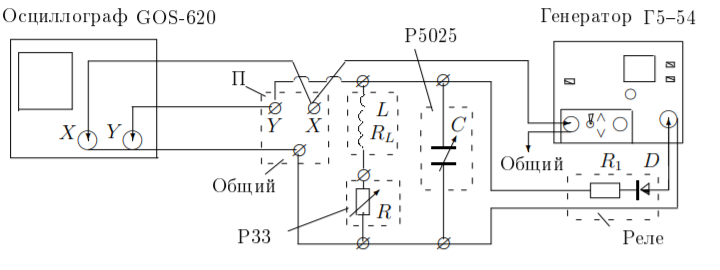
\includegraphics{Рис1.png}
	\caption{}
	\label{fig1}
\end{figure}


{\bfseries Экспериментальная установка.} На рис. \ref{fig1} приведена схема установки для исследования свободных
колебаний в контуре, содержащим постоянную индуктивность $L$ с активным сопротивлением $R_L$, а также переменное 
сопротивление $R$ и ёмкость $C$, выбираемые из соответствующих "магазинов". Картина колебаний наблюдается на экране осциллографа.

Для периодического возбуждения колебаний в контуре используется генератор импульсов. Каждый импульс заряжает конденсатор $C$, 
после чего в контуре возникают свободные затухающие колебания.Напряжение на конденсаторе поступает на вход $1(X)$ канала осциллографа, в напряжение на резисторе $2(X)$ - на вход канала $2(Y)$.
\newpage
{\bfseries Теоретическая подоплека.} 

Формула периода колебаний колебательного контура: 
\begin{equation} 
\begin{aligned} \label{period}
T = 2\pi\sqrt{LC}
\end{aligned}
\end{equation}
Формула для расчета логарифмического декремента затухания
\begin{equation} 
\begin{aligned} \label{logdek}
\Theta = \frac{1}{n}\ln\frac{U_k}{U_{k+n}}
\end{aligned}
\end{equation}
Формула для расчета сопротивления контура
\begin{equation} 
\begin{aligned} \label{Rsum}
R_{\text{конт}} = R + R_L,\text{ {  }   } R_L \approx 12 \text{ Ом}
\end{aligned}
\end{equation}
Формула для расчета критического сопротивления
\begin{equation} 
\begin{aligned} \label{Rcrit}
R_{\text{кр}} = 2\pi\sqrt{\frac{L}{C}}
\end{aligned}
\end{equation}
Формула для расчета критического сопротивления по МНК
\begin{equation} 
\begin{aligned} \label{MNK}
Y = A_{\text{МНК}}X+B_{\text{МНК}} \\
Y = \frac{1}{\Theta^2}, X = \frac{1}{R_{\text{конт}}^2}, A_{\text{МНК}} = \frac{R_{\text{кр}}^2}{4\pi^2}, B_{\text{МНК}} =  \frac{1}{4\pi^2} \\
R_{\text{кр}} = 2\pi\sqrt{A_{\text{МНК}}} \pm \frac{\pi}{\sqrt{A_{\text{МНК}}}}\delta A_{\text{МНК}}
\end{aligned}
\end{equation}
Экспериментальная и теоретическая формула для добротности контура
\begin{equation} 
\begin{aligned} \label{Dobr}
Q^\text{эксп}= \frac{\pi}{\Theta} \\
Q^\text{теор}= \frac{1}{R_\text{конт}}\sqrt{\frac{L}{C}}
\end{aligned}
\end{equation}
{\bfseries Результаты эксперимента.} С помощью формулы \ref{period} можно сравнить экспериментальные и теоретические значения для периодов колебаний. Результаты приведены на рисунке \ref{fig2}. Далее, подбором нужной картинке на осциллографе, было получено экспериментальное значение критического сопротивления $R_\text{кр}^\text{эксп, подбор} = 1000 \text{ Ом}$. Это же значение получено с помощью метода наименьших квадратов из линейного графика на рис. \ref{fig3} - $R_\text{кр}^\text{эксп, МНК} = 850 \pm 46 \text{ Ом}$  по формулам \ref{MNK}. Теоретическое значение получено из формулы \ref{Rcrit} - $R_\text{кр}^\text{теор} = 1369 \text{ Ом}$.
\begin{figure}[h!]
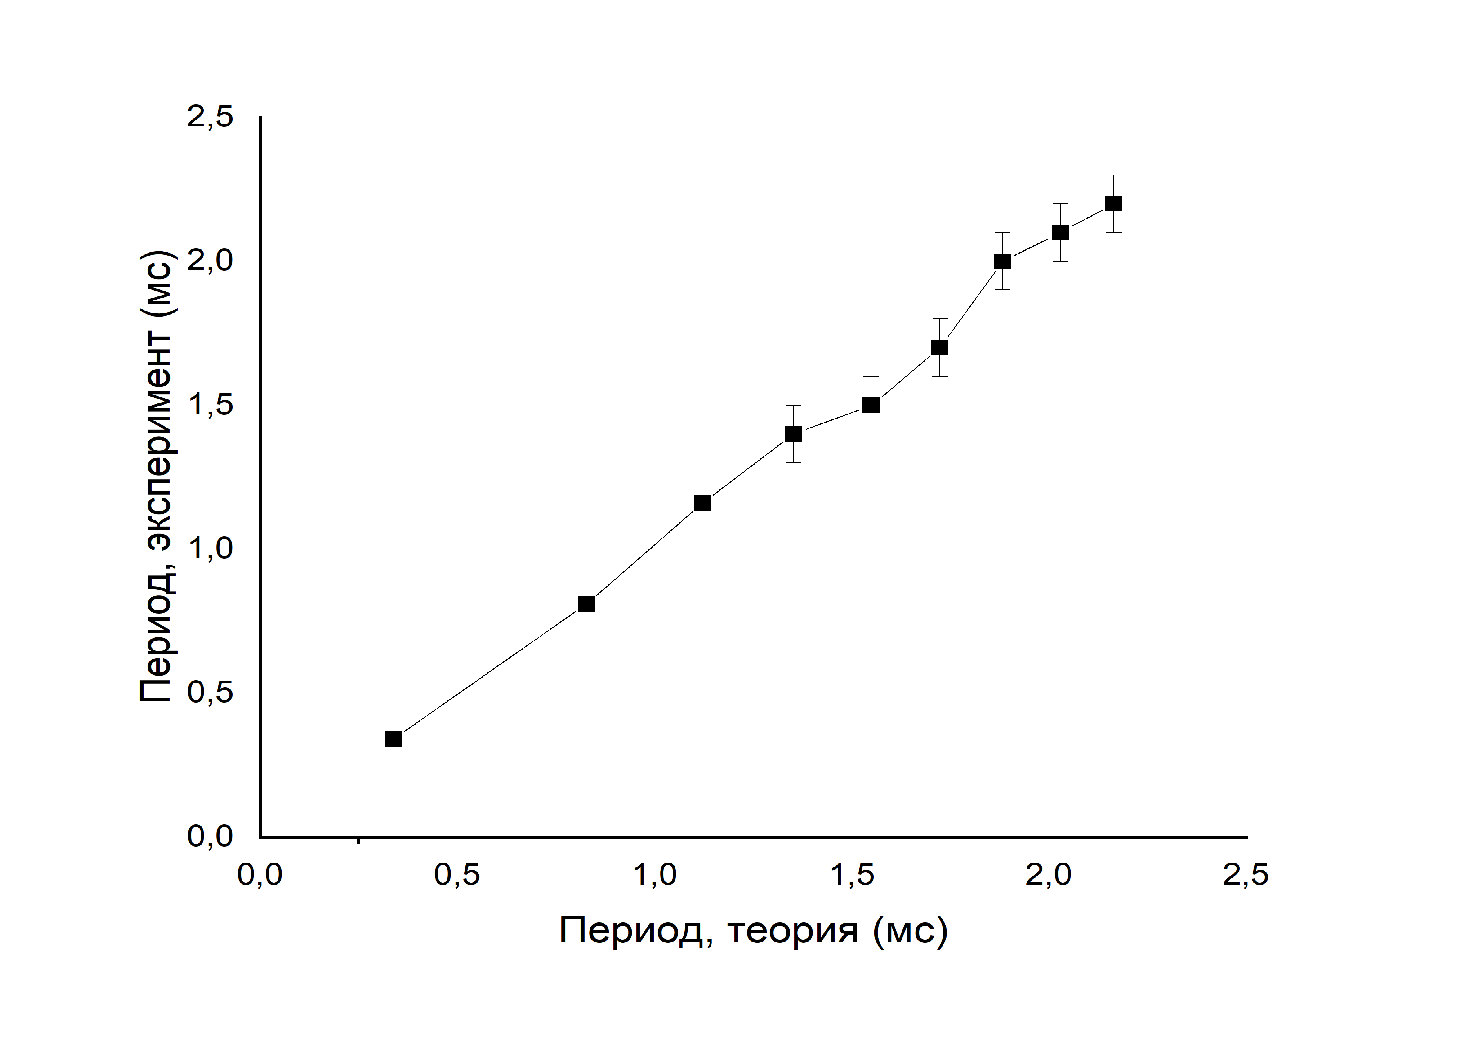
\includegraphics{Рис2.png}
\caption{}
\label{fig2}
\end{figure}
\begin{figure}[h!]
	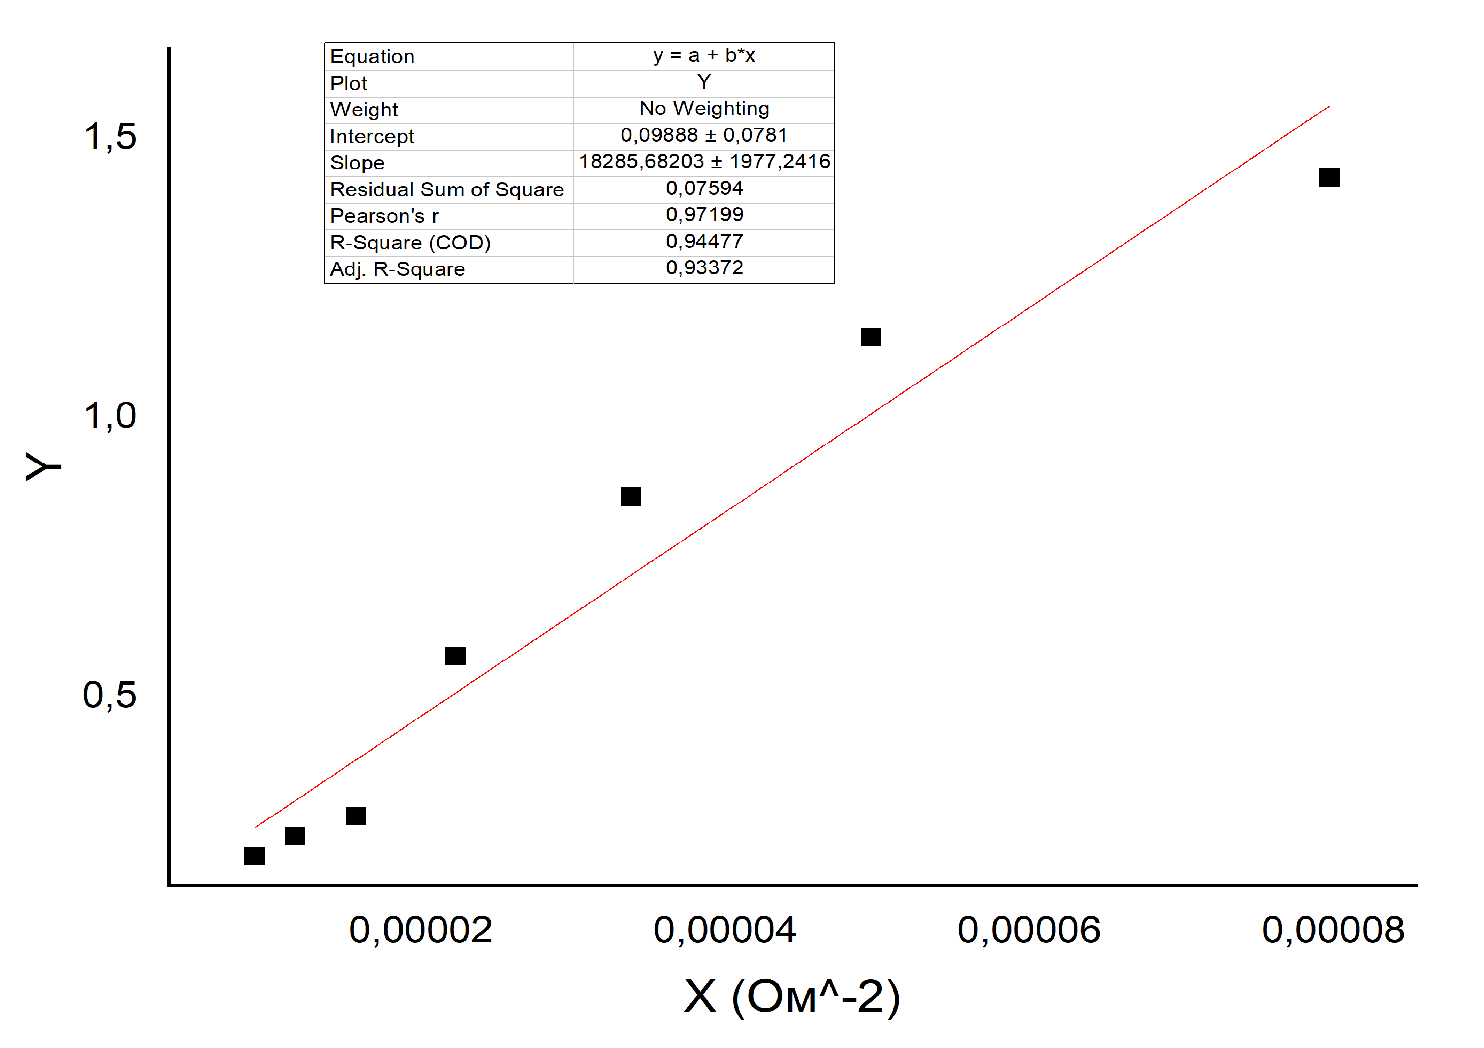
\includegraphics{Рис3.png}
	\caption{}
	\label{fig3}
\end{figure}
\newpage

В самом конце получены значения для добротности колебательного контура:

	\begin{table}[h]
		\begin{center}
		\begin{tabular}{|l|l|l|l|}
			\hline
		$Q_\text{max}^\text{эксп}$ & $Q_\text{min}^\text{эксп}$ & $Q_\text{max}^\text{теор}$ & $Q_\text{min}^\text{теор}$ \\ \hline
		3,75	&  1,45 & 6,01 & 2,03 \\ \hline
		\end{tabular}
	\end{center}
	\end{table}

\end{document}